% Created by tikzDevice version 0.7.0 on 2014-07-26 02:55:56
% !TEX encoding = UTF-8 Unicode
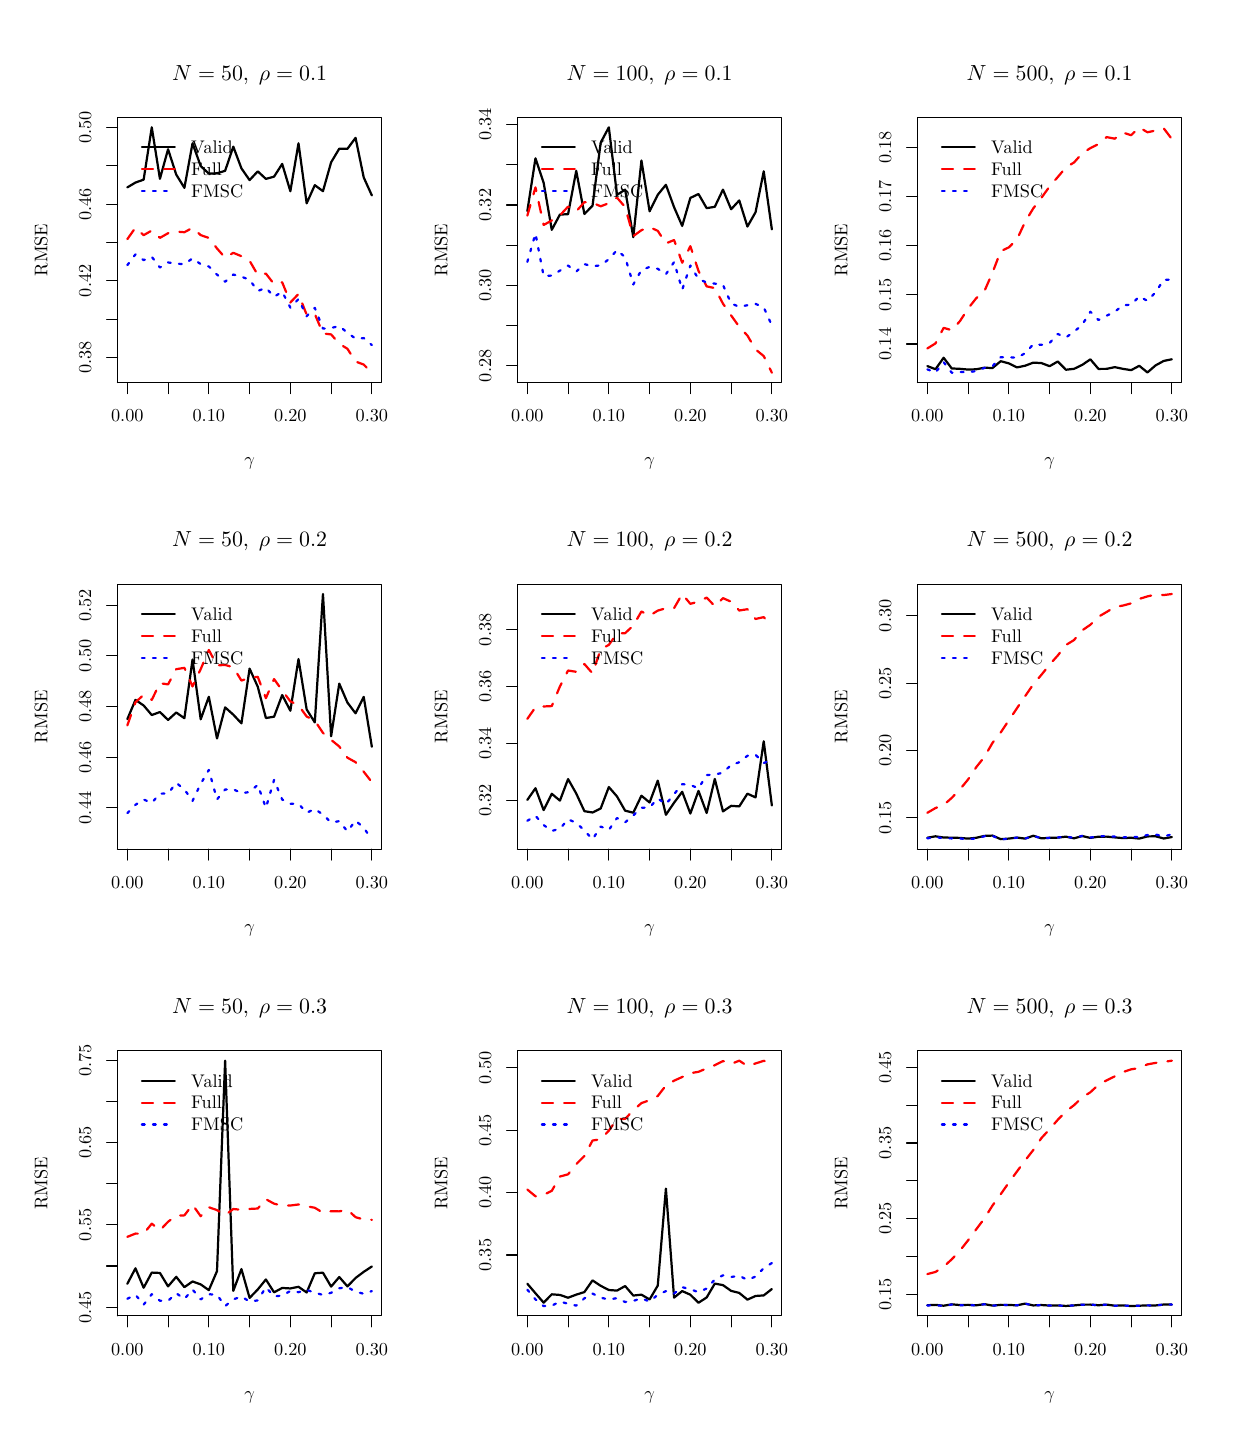
\begin{tikzpicture}[x=1pt,y=1pt]
\definecolor[named]{fillColor}{rgb}{1.00,1.00,1.00}
\path[use as bounding box,fill=fillColor,fill opacity=0.00] (0,0) rectangle (433.62,505.89);
\begin{scope}
\path[clip] ( 32.47,377.65) rectangle (127.91,473.42);
\definecolor[named]{drawColor}{rgb}{0.00,0.00,0.00}

\path[draw=drawColor,line width= 0.8pt,line join=round,line cap=round] ( 36.01,448.17) --
	( 38.95,449.92) --
	( 41.90,450.96) --
	( 44.84,469.87) --
	( 47.79,451.28) --
	( 50.73,461.95) --
	( 53.68,452.81) --
	( 56.63,448.00) --
	( 59.57,464.11) --
	( 62.52,455.87) --
	( 65.46,453.16) --
	( 68.41,453.26) --
	( 71.35,454.17) --
	( 74.30,462.89) --
	( 77.24,455.05) --
	( 80.19,450.80) --
	( 83.14,453.97) --
	( 86.08,451.24) --
	( 89.03,452.05) --
	( 91.97,456.65) --
	( 94.92,446.78) --
	( 97.86,464.11) --
	(100.81,442.41) --
	(103.75,448.98) --
	(106.70,446.80) --
	(109.65,457.24) --
	(112.59,462.15) --
	(115.54,462.11) --
	(118.48,466.07) --
	(121.43,451.77) --
	(124.37,445.26);
\end{scope}
\begin{scope}
\path[clip] (  0.00,  0.00) rectangle (433.62,505.89);
\definecolor[named]{drawColor}{rgb}{0.00,0.00,0.00}

\path[draw=drawColor,line width= 0.4pt,line join=round,line cap=round] ( 36.01,377.65) -- (124.37,377.65);

\path[draw=drawColor,line width= 0.4pt,line join=round,line cap=round] ( 36.01,377.65) -- ( 36.01,373.69);

\path[draw=drawColor,line width= 0.4pt,line join=round,line cap=round] ( 50.73,377.65) -- ( 50.73,373.69);

\path[draw=drawColor,line width= 0.4pt,line join=round,line cap=round] ( 65.46,377.65) -- ( 65.46,373.69);

\path[draw=drawColor,line width= 0.4pt,line join=round,line cap=round] ( 80.19,377.65) -- ( 80.19,373.69);

\path[draw=drawColor,line width= 0.4pt,line join=round,line cap=round] ( 94.92,377.65) -- ( 94.92,373.69);

\path[draw=drawColor,line width= 0.4pt,line join=round,line cap=round] (109.65,377.65) -- (109.65,373.69);

\path[draw=drawColor,line width= 0.4pt,line join=round,line cap=round] (124.37,377.65) -- (124.37,373.69);

\node[text=drawColor,anchor=base,inner sep=0pt, outer sep=0pt, scale=  0.66] at ( 36.01,363.40) {0.00};

\node[text=drawColor,anchor=base,inner sep=0pt, outer sep=0pt, scale=  0.66] at ( 65.46,363.40) {0.10};

\node[text=drawColor,anchor=base,inner sep=0pt, outer sep=0pt, scale=  0.66] at ( 94.92,363.40) {0.20};

\node[text=drawColor,anchor=base,inner sep=0pt, outer sep=0pt, scale=  0.66] at (124.37,363.40) {0.30};

\path[draw=drawColor,line width= 0.4pt,line join=round,line cap=round] ( 32.47,386.69) -- ( 32.47,469.81);

\path[draw=drawColor,line width= 0.4pt,line join=round,line cap=round] ( 32.47,386.69) -- ( 28.51,386.69);

\path[draw=drawColor,line width= 0.4pt,line join=round,line cap=round] ( 32.47,400.54) -- ( 28.51,400.54);

\path[draw=drawColor,line width= 0.4pt,line join=round,line cap=round] ( 32.47,414.40) -- ( 28.51,414.40);

\path[draw=drawColor,line width= 0.4pt,line join=round,line cap=round] ( 32.47,428.25) -- ( 28.51,428.25);

\path[draw=drawColor,line width= 0.4pt,line join=round,line cap=round] ( 32.47,442.11) -- ( 28.51,442.11);

\path[draw=drawColor,line width= 0.4pt,line join=round,line cap=round] ( 32.47,455.96) -- ( 28.51,455.96);

\path[draw=drawColor,line width= 0.4pt,line join=round,line cap=round] ( 32.47,469.81) -- ( 28.51,469.81);

\node[text=drawColor,rotate= 90.00,anchor=base,inner sep=0pt, outer sep=0pt, scale=  0.66] at ( 22.97,386.69) {0.38};

\node[text=drawColor,rotate= 90.00,anchor=base,inner sep=0pt, outer sep=0pt, scale=  0.66] at ( 22.97,414.40) {0.42};

\node[text=drawColor,rotate= 90.00,anchor=base,inner sep=0pt, outer sep=0pt, scale=  0.66] at ( 22.97,442.11) {0.46};

\node[text=drawColor,rotate= 90.00,anchor=base,inner sep=0pt, outer sep=0pt, scale=  0.66] at ( 22.97,469.81) {0.50};

\path[draw=drawColor,line width= 0.4pt,line join=round,line cap=round] ( 32.47,377.65) --
	(127.91,377.65) --
	(127.91,473.42) --
	( 32.47,473.42) --
	( 32.47,377.65);
\end{scope}
\begin{scope}
\path[clip] (  0.00,337.26) rectangle (144.54,505.89);
\definecolor[named]{drawColor}{rgb}{0.00,0.00,0.00}

\node[text=drawColor,anchor=base,inner sep=0pt, outer sep=0pt, scale=  0.79] at ( 80.19,486.92) {\bfseries $N=50, \;\rho=0.1$};

\node[text=drawColor,anchor=base,inner sep=0pt, outer sep=0pt, scale=  0.66] at ( 80.19,347.56) {$\gamma$};

\node[text=drawColor,rotate= 90.00,anchor=base,inner sep=0pt, outer sep=0pt, scale=  0.66] at (  7.13,425.53) {RMSE};
\end{scope}
\begin{scope}
\path[clip] ( 32.47,377.65) rectangle (127.91,473.42);
\definecolor[named]{drawColor}{rgb}{1.00,0.00,0.00}

\path[draw=drawColor,line width= 0.8pt,dash pattern=on 4pt off 4pt ,line join=round,line cap=round] ( 36.01,429.46) --
	( 38.95,433.63) --
	( 41.90,430.90) --
	( 44.84,432.59) --
	( 47.79,429.94) --
	( 50.73,431.61) --
	( 53.68,432.19) --
	( 56.63,431.97) --
	( 59.57,433.56) --
	( 62.52,430.92) --
	( 65.46,429.91) --
	( 68.41,426.11) --
	( 71.35,422.76) --
	( 74.30,424.53) --
	( 77.24,423.31) --
	( 80.19,421.66) --
	( 83.14,416.55) --
	( 86.08,417.02) --
	( 89.03,413.22) --
	( 91.97,413.88) --
	( 94.92,406.58) --
	( 97.86,409.67) --
	(100.81,402.20) --
	(103.75,402.43) --
	(106.70,395.39) --
	(109.65,395.04) --
	(112.59,391.68) --
	(115.54,389.86) --
	(118.48,385.25) --
	(121.43,384.15) --
	(124.37,381.20);
\definecolor[named]{drawColor}{rgb}{0.00,0.00,1.00}

\path[draw=drawColor,line width= 0.8pt,dash pattern=on 1pt off 3pt ,line join=round,line cap=round] ( 36.01,420.06) --
	( 38.95,423.99) --
	( 41.90,421.89) --
	( 44.84,423.09) --
	( 47.79,419.22) --
	( 50.73,421.05) --
	( 53.68,420.61) --
	( 56.63,420.43) --
	( 59.57,422.53) --
	( 62.52,420.44) --
	( 65.46,419.58) --
	( 68.41,416.66) --
	( 71.35,414.08) --
	( 74.30,416.68) --
	( 77.24,415.90) --
	( 80.19,414.78) --
	( 83.14,410.72) --
	( 86.08,411.91) --
	( 89.03,408.63) --
	( 91.97,410.45) --
	( 94.92,404.73) --
	( 97.86,407.82) --
	(100.81,401.62) --
	(103.75,404.64) --
	(106.70,397.13) --
	(109.65,397.38) --
	(112.59,398.06) --
	(115.54,395.67) --
	(118.48,393.51) --
	(121.43,393.72) --
	(124.37,391.19);
\definecolor[named]{drawColor}{rgb}{0.00,0.00,0.00}

\path[draw=drawColor,line width= 0.8pt,line join=round,line cap=round] ( 41.28,462.63) -- ( 53.16,462.63);
\definecolor[named]{drawColor}{rgb}{1.00,0.00,0.00}

\path[draw=drawColor,line width= 0.8pt,dash pattern=on 4pt off 4pt ,line join=round,line cap=round] ( 41.28,454.71) -- ( 53.16,454.71);
\definecolor[named]{drawColor}{rgb}{0.00,0.00,1.00}

\path[draw=drawColor,line width= 0.8pt,dash pattern=on 1pt off 3pt ,line join=round,line cap=round] ( 41.28,446.79) -- ( 53.16,446.79);
\definecolor[named]{drawColor}{rgb}{0.00,0.00,0.00}

\node[text=drawColor,anchor=base west,inner sep=0pt, outer sep=0pt, scale=  0.66] at ( 59.10,460.35) {Valid};

\node[text=drawColor,anchor=base west,inner sep=0pt, outer sep=0pt, scale=  0.66] at ( 59.10,452.43) {Full};

\node[text=drawColor,anchor=base west,inner sep=0pt, outer sep=0pt, scale=  0.66] at ( 59.10,444.51) {FMSC};
\end{scope}
\begin{scope}
\path[clip] (177.01,377.65) rectangle (272.45,473.42);
\definecolor[named]{drawColor}{rgb}{0.00,0.00,0.00}

\path[draw=drawColor,line width= 0.8pt,line join=round,line cap=round] (180.55,439.60) --
	(183.49,458.67) --
	(186.44,449.88) --
	(189.38,432.84) --
	(192.33,438.36) --
	(195.27,438.48) --
	(198.22,454.16) --
	(201.17,438.54) --
	(204.11,441.57) --
	(207.06,464.36) --
	(210.00,469.87) --
	(212.95,445.48) --
	(215.89,447.35) --
	(218.84,430.18) --
	(221.78,457.89) --
	(224.73,439.52) --
	(227.68,445.50) --
	(230.62,449.11) --
	(233.57,441.03) --
	(236.51,434.25) --
	(239.46,444.37) --
	(242.40,445.78) --
	(245.35,440.66) --
	(248.29,441.15) --
	(251.24,447.36) --
	(254.19,440.27) --
	(257.13,443.46) --
	(260.08,434.01) --
	(263.02,439.21) --
	(265.97,453.97) --
	(268.91,432.99);
\end{scope}
\begin{scope}
\path[clip] (  0.00,  0.00) rectangle (433.62,505.89);
\definecolor[named]{drawColor}{rgb}{0.00,0.00,0.00}

\path[draw=drawColor,line width= 0.4pt,line join=round,line cap=round] (180.55,377.65) -- (268.91,377.65);

\path[draw=drawColor,line width= 0.4pt,line join=round,line cap=round] (180.55,377.65) -- (180.55,373.69);

\path[draw=drawColor,line width= 0.4pt,line join=round,line cap=round] (195.27,377.65) -- (195.27,373.69);

\path[draw=drawColor,line width= 0.4pt,line join=round,line cap=round] (210.00,377.65) -- (210.00,373.69);

\path[draw=drawColor,line width= 0.4pt,line join=round,line cap=round] (224.73,377.65) -- (224.73,373.69);

\path[draw=drawColor,line width= 0.4pt,line join=round,line cap=round] (239.46,377.65) -- (239.46,373.69);

\path[draw=drawColor,line width= 0.4pt,line join=round,line cap=round] (254.19,377.65) -- (254.19,373.69);

\path[draw=drawColor,line width= 0.4pt,line join=round,line cap=round] (268.91,377.65) -- (268.91,373.69);

\node[text=drawColor,anchor=base,inner sep=0pt, outer sep=0pt, scale=  0.66] at (180.55,363.40) {0.00};

\node[text=drawColor,anchor=base,inner sep=0pt, outer sep=0pt, scale=  0.66] at (210.00,363.40) {0.10};

\node[text=drawColor,anchor=base,inner sep=0pt, outer sep=0pt, scale=  0.66] at (239.46,363.40) {0.20};

\node[text=drawColor,anchor=base,inner sep=0pt, outer sep=0pt, scale=  0.66] at (268.91,363.40) {0.30};

\path[draw=drawColor,line width= 0.4pt,line join=round,line cap=round] (177.01,383.70) -- (177.01,470.85);

\path[draw=drawColor,line width= 0.4pt,line join=round,line cap=round] (177.01,383.70) -- (173.05,383.70);

\path[draw=drawColor,line width= 0.4pt,line join=round,line cap=round] (177.01,398.23) -- (173.05,398.23);

\path[draw=drawColor,line width= 0.4pt,line join=round,line cap=round] (177.01,412.75) -- (173.05,412.75);

\path[draw=drawColor,line width= 0.4pt,line join=round,line cap=round] (177.01,427.28) -- (173.05,427.28);

\path[draw=drawColor,line width= 0.4pt,line join=round,line cap=round] (177.01,441.80) -- (173.05,441.80);

\path[draw=drawColor,line width= 0.4pt,line join=round,line cap=round] (177.01,456.33) -- (173.05,456.33);

\path[draw=drawColor,line width= 0.4pt,line join=round,line cap=round] (177.01,470.85) -- (173.05,470.85);

\node[text=drawColor,rotate= 90.00,anchor=base,inner sep=0pt, outer sep=0pt, scale=  0.66] at (167.51,383.70) {0.28};

\node[text=drawColor,rotate= 90.00,anchor=base,inner sep=0pt, outer sep=0pt, scale=  0.66] at (167.51,412.75) {0.30};

\node[text=drawColor,rotate= 90.00,anchor=base,inner sep=0pt, outer sep=0pt, scale=  0.66] at (167.51,441.80) {0.32};

\node[text=drawColor,rotate= 90.00,anchor=base,inner sep=0pt, outer sep=0pt, scale=  0.66] at (167.51,470.85) {0.34};

\path[draw=drawColor,line width= 0.4pt,line join=round,line cap=round] (177.01,377.65) --
	(272.45,377.65) --
	(272.45,473.42) --
	(177.01,473.42) --
	(177.01,377.65);
\end{scope}
\begin{scope}
\path[clip] (144.54,337.26) rectangle (289.08,505.89);
\definecolor[named]{drawColor}{rgb}{0.00,0.00,0.00}

\node[text=drawColor,anchor=base,inner sep=0pt, outer sep=0pt, scale=  0.79] at (224.73,486.92) {\bfseries $N=100, \;\rho=0.1$};

\node[text=drawColor,anchor=base,inner sep=0pt, outer sep=0pt, scale=  0.66] at (224.73,347.56) {$\gamma$};

\node[text=drawColor,rotate= 90.00,anchor=base,inner sep=0pt, outer sep=0pt, scale=  0.66] at (151.67,425.53) {RMSE};
\end{scope}
\begin{scope}
\path[clip] (177.01,377.65) rectangle (272.45,473.42);
\definecolor[named]{drawColor}{rgb}{1.00,0.00,0.00}

\path[draw=drawColor,line width= 0.8pt,dash pattern=on 4pt off 4pt ,line join=round,line cap=round] (180.55,437.96) --
	(183.49,448.17) --
	(186.44,434.59) --
	(189.38,436.22) --
	(192.33,438.07) --
	(195.27,441.22) --
	(198.22,439.51) --
	(201.17,442.84) --
	(204.11,442.60) --
	(207.06,441.34) --
	(210.00,442.46) --
	(212.95,444.47) --
	(215.89,441.06) --
	(218.84,430.57) --
	(221.78,432.70) --
	(224.73,433.81) --
	(227.68,432.47) --
	(230.62,427.92) --
	(233.57,429.15) --
	(236.51,420.94) --
	(239.46,426.92) --
	(242.40,417.99) --
	(245.35,412.40) --
	(248.29,411.78) --
	(251.24,406.17) --
	(254.19,401.90) --
	(257.13,397.80) --
	(260.08,394.62) --
	(263.02,389.63) --
	(265.97,387.21) --
	(268.91,381.20);
\definecolor[named]{drawColor}{rgb}{0.00,0.00,1.00}

\path[draw=drawColor,line width= 0.8pt,dash pattern=on 1pt off 3pt ,line join=round,line cap=round] (180.55,421.24) --
	(183.49,431.51) --
	(186.44,416.15) --
	(189.38,416.31) --
	(192.33,418.09) --
	(195.27,419.92) --
	(198.22,417.75) --
	(201.17,420.44) --
	(204.11,419.68) --
	(207.06,420.00) --
	(210.00,422.21) --
	(212.95,425.52) --
	(215.89,422.93) --
	(218.84,413.10) --
	(221.78,418.29) --
	(224.73,419.43) --
	(227.68,418.76) --
	(230.62,416.78) --
	(233.57,421.18) --
	(236.51,411.23) --
	(239.46,419.92) --
	(242.40,415.07) --
	(245.35,413.79) --
	(248.29,413.40) --
	(251.24,412.94) --
	(254.19,406.24) --
	(257.13,405.00) --
	(260.08,405.59) --
	(263.02,406.07) --
	(265.97,404.84) --
	(268.91,398.28);
\definecolor[named]{drawColor}{rgb}{0.00,0.00,0.00}

\path[draw=drawColor,line width= 0.8pt,line join=round,line cap=round] (185.82,462.63) -- (197.70,462.63);
\definecolor[named]{drawColor}{rgb}{1.00,0.00,0.00}

\path[draw=drawColor,line width= 0.8pt,dash pattern=on 4pt off 4pt ,line join=round,line cap=round] (185.82,454.71) -- (197.70,454.71);
\definecolor[named]{drawColor}{rgb}{0.00,0.00,1.00}

\path[draw=drawColor,line width= 0.8pt,dash pattern=on 1pt off 3pt ,line join=round,line cap=round] (185.82,446.79) -- (197.70,446.79);
\definecolor[named]{drawColor}{rgb}{0.00,0.00,0.00}

\node[text=drawColor,anchor=base west,inner sep=0pt, outer sep=0pt, scale=  0.66] at (203.64,460.35) {Valid};

\node[text=drawColor,anchor=base west,inner sep=0pt, outer sep=0pt, scale=  0.66] at (203.64,452.43) {Full};

\node[text=drawColor,anchor=base west,inner sep=0pt, outer sep=0pt, scale=  0.66] at (203.64,444.51) {FMSC};
\end{scope}
\begin{scope}
\path[clip] (321.55,377.65) rectangle (416.99,473.42);
\definecolor[named]{drawColor}{rgb}{0.00,0.00,0.00}

\path[draw=drawColor,line width= 0.8pt,line join=round,line cap=round] (325.09,383.60) --
	(328.03,382.47) --
	(330.98,386.61) --
	(333.92,382.74) --
	(336.87,382.61) --
	(339.81,382.34) --
	(342.76,382.45) --
	(345.71,383.01) --
	(348.65,382.90) --
	(351.60,385.37) --
	(354.54,384.58) --
	(357.49,383.12) --
	(360.43,383.73) --
	(363.38,384.85) --
	(366.32,384.69) --
	(369.27,383.56) --
	(372.22,385.26) --
	(375.16,382.28) --
	(378.11,382.61) --
	(381.05,384.03) --
	(384.00,386.04) --
	(386.94,382.58) --
	(389.89,382.60) --
	(392.83,383.22) --
	(395.78,382.60) --
	(398.73,382.13) --
	(401.67,383.70) --
	(404.62,381.30) --
	(407.56,383.85) --
	(410.51,385.46) --
	(413.45,386.06);
\end{scope}
\begin{scope}
\path[clip] (  0.00,  0.00) rectangle (433.62,505.89);
\definecolor[named]{drawColor}{rgb}{0.00,0.00,0.00}

\path[draw=drawColor,line width= 0.4pt,line join=round,line cap=round] (325.09,377.65) -- (413.45,377.65);

\path[draw=drawColor,line width= 0.4pt,line join=round,line cap=round] (325.09,377.65) -- (325.09,373.69);

\path[draw=drawColor,line width= 0.4pt,line join=round,line cap=round] (339.81,377.65) -- (339.81,373.69);

\path[draw=drawColor,line width= 0.4pt,line join=round,line cap=round] (354.54,377.65) -- (354.54,373.69);

\path[draw=drawColor,line width= 0.4pt,line join=round,line cap=round] (369.27,377.65) -- (369.27,373.69);

\path[draw=drawColor,line width= 0.4pt,line join=round,line cap=round] (384.00,377.65) -- (384.00,373.69);

\path[draw=drawColor,line width= 0.4pt,line join=round,line cap=round] (398.73,377.65) -- (398.73,373.69);

\path[draw=drawColor,line width= 0.4pt,line join=round,line cap=round] (413.45,377.65) -- (413.45,373.69);

\node[text=drawColor,anchor=base,inner sep=0pt, outer sep=0pt, scale=  0.66] at (325.09,363.40) {0.00};

\node[text=drawColor,anchor=base,inner sep=0pt, outer sep=0pt, scale=  0.66] at (354.54,363.40) {0.10};

\node[text=drawColor,anchor=base,inner sep=0pt, outer sep=0pt, scale=  0.66] at (384.00,363.40) {0.20};

\node[text=drawColor,anchor=base,inner sep=0pt, outer sep=0pt, scale=  0.66] at (413.45,363.40) {0.30};

\path[draw=drawColor,line width= 0.4pt,line join=round,line cap=round] (321.55,391.57) -- (321.55,462.73);

\path[draw=drawColor,line width= 0.4pt,line join=round,line cap=round] (321.55,391.57) -- (317.59,391.57);

\path[draw=drawColor,line width= 0.4pt,line join=round,line cap=round] (321.55,409.36) -- (317.59,409.36);

\path[draw=drawColor,line width= 0.4pt,line join=round,line cap=round] (321.55,427.15) -- (317.59,427.15);

\path[draw=drawColor,line width= 0.4pt,line join=round,line cap=round] (321.55,444.94) -- (317.59,444.94);

\path[draw=drawColor,line width= 0.4pt,line join=round,line cap=round] (321.55,462.73) -- (317.59,462.73);

\node[text=drawColor,rotate= 90.00,anchor=base,inner sep=0pt, outer sep=0pt, scale=  0.66] at (312.05,391.57) {0.14};

\node[text=drawColor,rotate= 90.00,anchor=base,inner sep=0pt, outer sep=0pt, scale=  0.66] at (312.05,409.36) {0.15};

\node[text=drawColor,rotate= 90.00,anchor=base,inner sep=0pt, outer sep=0pt, scale=  0.66] at (312.05,427.15) {0.16};

\node[text=drawColor,rotate= 90.00,anchor=base,inner sep=0pt, outer sep=0pt, scale=  0.66] at (312.05,444.94) {0.17};

\node[text=drawColor,rotate= 90.00,anchor=base,inner sep=0pt, outer sep=0pt, scale=  0.66] at (312.05,462.73) {0.18};

\path[draw=drawColor,line width= 0.4pt,line join=round,line cap=round] (321.55,377.65) --
	(416.99,377.65) --
	(416.99,473.42) --
	(321.55,473.42) --
	(321.55,377.65);
\end{scope}
\begin{scope}
\path[clip] (289.08,337.26) rectangle (433.62,505.89);
\definecolor[named]{drawColor}{rgb}{0.00,0.00,0.00}

\node[text=drawColor,anchor=base,inner sep=0pt, outer sep=0pt, scale=  0.79] at (369.27,486.92) {\bfseries $N=500, \;\rho=0.1$};

\node[text=drawColor,anchor=base,inner sep=0pt, outer sep=0pt, scale=  0.66] at (369.27,347.56) {$\gamma$};

\node[text=drawColor,rotate= 90.00,anchor=base,inner sep=0pt, outer sep=0pt, scale=  0.66] at (296.21,425.53) {RMSE};
\end{scope}
\begin{scope}
\path[clip] (321.55,377.65) rectangle (416.99,473.42);
\definecolor[named]{drawColor}{rgb}{1.00,0.00,0.00}

\path[draw=drawColor,line width= 0.8pt,dash pattern=on 4pt off 4pt ,line join=round,line cap=round] (325.09,389.98) --
	(328.03,391.78) --
	(330.98,397.42) --
	(333.92,396.56) --
	(336.87,399.84) --
	(339.81,404.38) --
	(342.76,408.13) --
	(345.71,410.69) --
	(348.65,417.41) --
	(351.60,425.12) --
	(354.54,426.50) --
	(357.49,429.40) --
	(360.43,435.73) --
	(363.38,440.60) --
	(366.32,444.42) --
	(369.27,448.51) --
	(372.22,451.91) --
	(375.16,455.39) --
	(378.11,457.18) --
	(381.05,460.48) --
	(384.00,462.36) --
	(386.94,463.82) --
	(389.89,466.35) --
	(392.83,465.77) --
	(395.78,467.97) --
	(398.73,467.03) --
	(401.67,469.87) --
	(404.62,468.09) --
	(407.56,468.70) --
	(410.51,469.51) --
	(413.45,465.62);
\definecolor[named]{drawColor}{rgb}{0.00,0.00,1.00}

\path[draw=drawColor,line width= 0.8pt,dash pattern=on 1pt off 3pt ,line join=round,line cap=round] (325.09,382.42) --
	(328.03,381.28) --
	(330.98,385.02) --
	(333.92,381.20) --
	(336.87,381.47) --
	(339.81,381.37) --
	(342.76,381.81) --
	(345.71,382.94) --
	(348.65,383.57) --
	(351.60,386.81) --
	(354.54,386.83) --
	(357.49,386.58) --
	(360.43,388.27) --
	(363.38,391.48) --
	(366.32,391.29) --
	(369.27,391.93) --
	(372.22,395.20) --
	(375.16,393.94) --
	(378.11,396.02) --
	(381.05,398.55) --
	(384.00,403.23) --
	(386.94,400.25) --
	(389.89,401.82) --
	(392.83,403.24) --
	(395.78,405.59) --
	(398.73,405.78) --
	(401.67,408.80) --
	(404.62,407.16) --
	(407.56,410.29) --
	(410.51,414.78) --
	(413.45,414.87);
\definecolor[named]{drawColor}{rgb}{0.00,0.00,0.00}

\path[draw=drawColor,line width= 0.8pt,line join=round,line cap=round] (330.36,462.63) -- (342.24,462.63);
\definecolor[named]{drawColor}{rgb}{1.00,0.00,0.00}

\path[draw=drawColor,line width= 0.8pt,dash pattern=on 4pt off 4pt ,line join=round,line cap=round] (330.36,454.71) -- (342.24,454.71);
\definecolor[named]{drawColor}{rgb}{0.00,0.00,1.00}

\path[draw=drawColor,line width= 0.8pt,dash pattern=on 1pt off 3pt ,line join=round,line cap=round] (330.36,446.79) -- (342.24,446.79);
\definecolor[named]{drawColor}{rgb}{0.00,0.00,0.00}

\node[text=drawColor,anchor=base west,inner sep=0pt, outer sep=0pt, scale=  0.66] at (348.18,460.35) {Valid};

\node[text=drawColor,anchor=base west,inner sep=0pt, outer sep=0pt, scale=  0.66] at (348.18,452.43) {Full};

\node[text=drawColor,anchor=base west,inner sep=0pt, outer sep=0pt, scale=  0.66] at (348.18,444.51) {FMSC};
\end{scope}
\begin{scope}
\path[clip] ( 32.47,209.02) rectangle (127.91,304.79);
\definecolor[named]{drawColor}{rgb}{0.00,0.00,0.00}

\path[draw=drawColor,line width= 0.8pt,line join=round,line cap=round] ( 36.01,256.01) --
	( 38.95,262.97) --
	( 41.90,260.97) --
	( 44.84,257.51) --
	( 47.79,258.59) --
	( 50.73,255.73) --
	( 53.68,258.42) --
	( 56.63,256.36) --
	( 59.57,277.59) --
	( 62.52,255.98) --
	( 65.46,264.10) --
	( 68.41,249.05) --
	( 71.35,260.28) --
	( 74.30,257.64) --
	( 77.24,254.50) --
	( 80.19,274.27) --
	( 83.14,267.74) --
	( 86.08,256.43) --
	( 89.03,256.91) --
	( 91.97,264.73) --
	( 94.92,259.07) --
	( 97.86,277.72) --
	(100.81,259.54) --
	(103.75,254.84) --
	(106.70,301.24) --
	(109.65,249.85) --
	(112.59,268.86) --
	(115.54,262.01) --
	(118.48,258.13) --
	(121.43,264.08) --
	(124.37,246.05);
\end{scope}
\begin{scope}
\path[clip] (  0.00,  0.00) rectangle (433.62,505.89);
\definecolor[named]{drawColor}{rgb}{0.00,0.00,0.00}

\path[draw=drawColor,line width= 0.4pt,line join=round,line cap=round] ( 36.01,209.02) -- (124.37,209.02);

\path[draw=drawColor,line width= 0.4pt,line join=round,line cap=round] ( 36.01,209.02) -- ( 36.01,205.06);

\path[draw=drawColor,line width= 0.4pt,line join=round,line cap=round] ( 50.73,209.02) -- ( 50.73,205.06);

\path[draw=drawColor,line width= 0.4pt,line join=round,line cap=round] ( 65.46,209.02) -- ( 65.46,205.06);

\path[draw=drawColor,line width= 0.4pt,line join=round,line cap=round] ( 80.19,209.02) -- ( 80.19,205.06);

\path[draw=drawColor,line width= 0.4pt,line join=round,line cap=round] ( 94.92,209.02) -- ( 94.92,205.06);

\path[draw=drawColor,line width= 0.4pt,line join=round,line cap=round] (109.65,209.02) -- (109.65,205.06);

\path[draw=drawColor,line width= 0.4pt,line join=round,line cap=round] (124.37,209.02) -- (124.37,205.06);

\node[text=drawColor,anchor=base,inner sep=0pt, outer sep=0pt, scale=  0.66] at ( 36.01,194.77) {0.00};

\node[text=drawColor,anchor=base,inner sep=0pt, outer sep=0pt, scale=  0.66] at ( 65.46,194.77) {0.10};

\node[text=drawColor,anchor=base,inner sep=0pt, outer sep=0pt, scale=  0.66] at ( 94.92,194.77) {0.20};

\node[text=drawColor,anchor=base,inner sep=0pt, outer sep=0pt, scale=  0.66] at (124.37,194.77) {0.30};

\path[draw=drawColor,line width= 0.4pt,line join=round,line cap=round] ( 32.47,223.95) -- ( 32.47,297.21);

\path[draw=drawColor,line width= 0.4pt,line join=round,line cap=round] ( 32.47,223.95) -- ( 28.51,223.95);

\path[draw=drawColor,line width= 0.4pt,line join=round,line cap=round] ( 32.47,242.27) -- ( 28.51,242.27);

\path[draw=drawColor,line width= 0.4pt,line join=round,line cap=round] ( 32.47,260.58) -- ( 28.51,260.58);

\path[draw=drawColor,line width= 0.4pt,line join=round,line cap=round] ( 32.47,278.90) -- ( 28.51,278.90);

\path[draw=drawColor,line width= 0.4pt,line join=round,line cap=round] ( 32.47,297.21) -- ( 28.51,297.21);

\node[text=drawColor,rotate= 90.00,anchor=base,inner sep=0pt, outer sep=0pt, scale=  0.66] at ( 22.97,223.95) {0.44};

\node[text=drawColor,rotate= 90.00,anchor=base,inner sep=0pt, outer sep=0pt, scale=  0.66] at ( 22.97,242.27) {0.46};

\node[text=drawColor,rotate= 90.00,anchor=base,inner sep=0pt, outer sep=0pt, scale=  0.66] at ( 22.97,260.58) {0.48};

\node[text=drawColor,rotate= 90.00,anchor=base,inner sep=0pt, outer sep=0pt, scale=  0.66] at ( 22.97,278.90) {0.50};

\node[text=drawColor,rotate= 90.00,anchor=base,inner sep=0pt, outer sep=0pt, scale=  0.66] at ( 22.97,297.21) {0.52};

\path[draw=drawColor,line width= 0.4pt,line join=round,line cap=round] ( 32.47,209.02) --
	(127.91,209.02) --
	(127.91,304.79) --
	( 32.47,304.79) --
	( 32.47,209.02);
\end{scope}
\begin{scope}
\path[clip] (  0.00,168.63) rectangle (144.54,337.26);
\definecolor[named]{drawColor}{rgb}{0.00,0.00,0.00}

\node[text=drawColor,anchor=base,inner sep=0pt, outer sep=0pt, scale=  0.79] at ( 80.19,318.29) {\bfseries $N=50, \;\rho=0.2$};

\node[text=drawColor,anchor=base,inner sep=0pt, outer sep=0pt, scale=  0.66] at ( 80.19,178.93) {$\gamma$};

\node[text=drawColor,rotate= 90.00,anchor=base,inner sep=0pt, outer sep=0pt, scale=  0.66] at (  7.13,256.90) {RMSE};
\end{scope}
\begin{scope}
\path[clip] ( 32.47,209.02) rectangle (127.91,304.79);
\definecolor[named]{drawColor}{rgb}{1.00,0.00,0.00}

\path[draw=drawColor,line width= 0.8pt,dash pattern=on 4pt off 4pt ,line join=round,line cap=round] ( 36.01,253.76) --
	( 38.95,262.11) --
	( 41.90,264.81) --
	( 44.84,263.01) --
	( 47.79,269.01) --
	( 50.73,268.59) --
	( 53.68,274.08) --
	( 56.63,274.57) --
	( 59.57,267.84) --
	( 62.52,274.09) --
	( 65.46,281.02) --
	( 68.41,275.44) --
	( 71.35,275.61) --
	( 74.30,274.76) --
	( 77.24,269.96) --
	( 80.19,270.95) --
	( 83.14,271.32) --
	( 86.08,263.60) --
	( 89.03,270.50) --
	( 91.97,266.38) --
	( 94.92,262.46) --
	( 97.86,261.03) --
	(100.81,256.98) --
	(103.75,255.49) --
	(106.70,251.06) --
	(109.65,248.55) --
	(112.59,246.14) --
	(115.54,242.10) --
	(118.48,240.47) --
	(121.43,237.02) --
	(124.37,233.24);
\definecolor[named]{drawColor}{rgb}{0.00,0.00,1.00}

\path[draw=drawColor,line width= 0.8pt,dash pattern=on 1pt off 3pt ,line join=round,line cap=round] ( 36.01,222.06) --
	( 38.95,225.07) --
	( 41.90,226.98) --
	( 44.84,225.77) --
	( 47.79,229.11) --
	( 50.73,229.13) --
	( 53.68,233.00) --
	( 56.63,230.64) --
	( 59.57,226.47) --
	( 62.52,232.65) --
	( 65.46,237.68) --
	( 68.41,227.01) --
	( 71.35,230.59) --
	( 74.30,230.71) --
	( 77.24,229.25) --
	( 80.19,229.70) --
	( 83.14,232.29) --
	( 86.08,223.96) --
	( 89.03,234.06) --
	( 91.97,226.98) --
	( 94.92,225.43) --
	( 97.86,225.46) --
	(100.81,222.19) --
	(103.75,223.57) --
	(106.70,221.53) --
	(109.65,218.65) --
	(112.59,219.18) --
	(115.54,215.47) --
	(118.48,219.37) --
	(121.43,216.75) --
	(124.37,212.57);
\definecolor[named]{drawColor}{rgb}{0.00,0.00,0.00}

\path[draw=drawColor,line width= 0.8pt,line join=round,line cap=round] ( 41.28,294.00) -- ( 53.16,294.00);
\definecolor[named]{drawColor}{rgb}{1.00,0.00,0.00}

\path[draw=drawColor,line width= 0.8pt,dash pattern=on 4pt off 4pt ,line join=round,line cap=round] ( 41.28,286.08) -- ( 53.16,286.08);
\definecolor[named]{drawColor}{rgb}{0.00,0.00,1.00}

\path[draw=drawColor,line width= 0.8pt,dash pattern=on 1pt off 3pt ,line join=round,line cap=round] ( 41.28,278.16) -- ( 53.16,278.16);
\definecolor[named]{drawColor}{rgb}{0.00,0.00,0.00}

\node[text=drawColor,anchor=base west,inner sep=0pt, outer sep=0pt, scale=  0.66] at ( 59.10,291.72) {Valid};

\node[text=drawColor,anchor=base west,inner sep=0pt, outer sep=0pt, scale=  0.66] at ( 59.10,283.80) {Full};

\node[text=drawColor,anchor=base west,inner sep=0pt, outer sep=0pt, scale=  0.66] at ( 59.10,275.88) {FMSC};
\end{scope}
\begin{scope}
\path[clip] (177.01,209.02) rectangle (272.45,304.79);
\definecolor[named]{drawColor}{rgb}{0.00,0.00,0.00}

\path[draw=drawColor,line width= 0.8pt,line join=round,line cap=round] (180.55,226.83) --
	(183.49,231.06) --
	(186.44,223.16) --
	(189.38,229.05) --
	(192.33,226.59) --
	(195.27,234.37) --
	(198.22,229.15) --
	(201.17,222.77) --
	(204.11,222.29) --
	(207.06,223.76) --
	(210.00,231.49) --
	(212.95,228.10) --
	(215.89,222.95) --
	(218.84,222.22) --
	(221.78,228.35) --
	(224.73,225.91) --
	(227.68,233.81) --
	(230.62,221.45) --
	(233.57,225.83) --
	(236.51,229.77) --
	(239.46,221.91) --
	(242.40,230.11) --
	(245.35,222.10) --
	(248.29,234.41) --
	(251.24,222.69) --
	(254.19,224.70) --
	(257.13,224.49) --
	(260.08,229.09) --
	(263.02,227.75) --
	(265.97,248.03) --
	(268.91,224.83);
\end{scope}
\begin{scope}
\path[clip] (  0.00,  0.00) rectangle (433.62,505.89);
\definecolor[named]{drawColor}{rgb}{0.00,0.00,0.00}

\path[draw=drawColor,line width= 0.4pt,line join=round,line cap=round] (180.55,209.02) -- (268.91,209.02);

\path[draw=drawColor,line width= 0.4pt,line join=round,line cap=round] (180.55,209.02) -- (180.55,205.06);

\path[draw=drawColor,line width= 0.4pt,line join=round,line cap=round] (195.27,209.02) -- (195.27,205.06);

\path[draw=drawColor,line width= 0.4pt,line join=round,line cap=round] (210.00,209.02) -- (210.00,205.06);

\path[draw=drawColor,line width= 0.4pt,line join=round,line cap=round] (224.73,209.02) -- (224.73,205.06);

\path[draw=drawColor,line width= 0.4pt,line join=round,line cap=round] (239.46,209.02) -- (239.46,205.06);

\path[draw=drawColor,line width= 0.4pt,line join=round,line cap=round] (254.19,209.02) -- (254.19,205.06);

\path[draw=drawColor,line width= 0.4pt,line join=round,line cap=round] (268.91,209.02) -- (268.91,205.06);

\node[text=drawColor,anchor=base,inner sep=0pt, outer sep=0pt, scale=  0.66] at (180.55,194.77) {0.00};

\node[text=drawColor,anchor=base,inner sep=0pt, outer sep=0pt, scale=  0.66] at (210.00,194.77) {0.10};

\node[text=drawColor,anchor=base,inner sep=0pt, outer sep=0pt, scale=  0.66] at (239.46,194.77) {0.20};

\node[text=drawColor,anchor=base,inner sep=0pt, outer sep=0pt, scale=  0.66] at (268.91,194.77) {0.30};

\path[draw=drawColor,line width= 0.4pt,line join=round,line cap=round] (177.01,226.59) -- (177.01,288.30);

\path[draw=drawColor,line width= 0.4pt,line join=round,line cap=round] (177.01,226.59) -- (173.05,226.59);

\path[draw=drawColor,line width= 0.4pt,line join=round,line cap=round] (177.01,247.16) -- (173.05,247.16);

\path[draw=drawColor,line width= 0.4pt,line join=round,line cap=round] (177.01,267.73) -- (173.05,267.73);

\path[draw=drawColor,line width= 0.4pt,line join=round,line cap=round] (177.01,288.30) -- (173.05,288.30);

\node[text=drawColor,rotate= 90.00,anchor=base,inner sep=0pt, outer sep=0pt, scale=  0.66] at (167.51,226.59) {0.32};

\node[text=drawColor,rotate= 90.00,anchor=base,inner sep=0pt, outer sep=0pt, scale=  0.66] at (167.51,247.16) {0.34};

\node[text=drawColor,rotate= 90.00,anchor=base,inner sep=0pt, outer sep=0pt, scale=  0.66] at (167.51,267.73) {0.36};

\node[text=drawColor,rotate= 90.00,anchor=base,inner sep=0pt, outer sep=0pt, scale=  0.66] at (167.51,288.30) {0.38};

\path[draw=drawColor,line width= 0.4pt,line join=round,line cap=round] (177.01,209.02) --
	(272.45,209.02) --
	(272.45,304.79) --
	(177.01,304.79) --
	(177.01,209.02);
\end{scope}
\begin{scope}
\path[clip] (144.54,168.63) rectangle (289.08,337.26);
\definecolor[named]{drawColor}{rgb}{0.00,0.00,0.00}

\node[text=drawColor,anchor=base,inner sep=0pt, outer sep=0pt, scale=  0.79] at (224.73,318.29) {\bfseries $N=100, \;\rho=0.2$};

\node[text=drawColor,anchor=base,inner sep=0pt, outer sep=0pt, scale=  0.66] at (224.73,178.93) {$\gamma$};

\node[text=drawColor,rotate= 90.00,anchor=base,inner sep=0pt, outer sep=0pt, scale=  0.66] at (151.67,256.90) {RMSE};
\end{scope}
\begin{scope}
\path[clip] (177.01,209.02) rectangle (272.45,304.79);
\definecolor[named]{drawColor}{rgb}{1.00,0.00,0.00}

\path[draw=drawColor,line width= 0.8pt,dash pattern=on 4pt off 4pt ,line join=round,line cap=round] (180.55,256.13) --
	(183.49,260.31) --
	(186.44,260.60) --
	(189.38,260.74) --
	(192.33,267.86) --
	(195.27,273.59) --
	(198.22,273.13) --
	(201.17,275.93) --
	(204.11,272.56) --
	(207.06,281.26) --
	(210.00,282.86) --
	(212.95,286.96) --
	(215.89,287.09) --
	(218.84,289.85) --
	(221.78,294.93) --
	(224.73,293.40) --
	(227.68,295.24) --
	(230.62,296.10) --
	(233.57,296.11) --
	(236.51,301.24) --
	(239.46,297.69) --
	(242.40,298.50) --
	(245.35,299.95) --
	(248.29,296.85) --
	(251.24,299.75) --
	(254.19,298.45) --
	(257.13,295.28) --
	(260.08,295.75) --
	(263.02,292.22) --
	(265.97,292.89) --
	(268.91,289.53);
\definecolor[named]{drawColor}{rgb}{0.00,0.00,1.00}

\path[draw=drawColor,line width= 0.8pt,dash pattern=on 1pt off 3pt ,line join=round,line cap=round] (180.55,219.29) --
	(183.49,221.10) --
	(186.44,217.76) --
	(189.38,215.62) --
	(192.33,216.44) --
	(195.27,219.81) --
	(198.22,218.57) --
	(201.17,215.80) --
	(204.11,212.57) --
	(207.06,217.22) --
	(210.00,215.98) --
	(212.95,220.29) --
	(215.89,218.74) --
	(218.84,221.25) --
	(221.78,224.01) --
	(224.73,224.11) --
	(227.68,227.37) --
	(230.62,225.29) --
	(233.57,228.89) --
	(236.51,232.54) --
	(239.46,232.24) --
	(242.40,231.03) --
	(245.35,235.83) --
	(248.29,235.98) --
	(251.24,236.69) --
	(254.19,239.46) --
	(257.13,240.45) --
	(260.08,242.79) --
	(263.02,243.14) --
	(265.97,240.17) --
	(268.91,241.42);
\definecolor[named]{drawColor}{rgb}{0.00,0.00,0.00}

\path[draw=drawColor,line width= 0.8pt,line join=round,line cap=round] (185.82,294.00) -- (197.70,294.00);
\definecolor[named]{drawColor}{rgb}{1.00,0.00,0.00}

\path[draw=drawColor,line width= 0.8pt,dash pattern=on 4pt off 4pt ,line join=round,line cap=round] (185.82,286.08) -- (197.70,286.08);
\definecolor[named]{drawColor}{rgb}{0.00,0.00,1.00}

\path[draw=drawColor,line width= 0.8pt,dash pattern=on 1pt off 3pt ,line join=round,line cap=round] (185.82,278.16) -- (197.70,278.16);
\definecolor[named]{drawColor}{rgb}{0.00,0.00,0.00}

\node[text=drawColor,anchor=base west,inner sep=0pt, outer sep=0pt, scale=  0.66] at (203.64,291.72) {Valid};

\node[text=drawColor,anchor=base west,inner sep=0pt, outer sep=0pt, scale=  0.66] at (203.64,283.80) {Full};

\node[text=drawColor,anchor=base west,inner sep=0pt, outer sep=0pt, scale=  0.66] at (203.64,275.88) {FMSC};
\end{scope}
\begin{scope}
\path[clip] (321.55,209.02) rectangle (416.99,304.79);
\definecolor[named]{drawColor}{rgb}{0.00,0.00,0.00}

\path[draw=drawColor,line width= 0.8pt,line join=round,line cap=round] (325.09,213.18) --
	(328.03,213.68) --
	(330.98,213.25) --
	(333.92,213.19) --
	(336.87,213.11) --
	(339.81,212.85) --
	(342.76,213.15) --
	(345.71,213.84) --
	(348.65,213.95) --
	(351.60,212.66) --
	(354.54,212.87) --
	(357.49,213.23) --
	(360.43,212.86) --
	(363.38,213.88) --
	(366.32,212.95) --
	(369.27,213.13) --
	(372.22,213.21) --
	(375.16,213.56) --
	(378.11,212.96) --
	(381.05,213.78) --
	(384.00,213.11) --
	(386.94,213.54) --
	(389.89,213.57) --
	(392.83,213.29) --
	(395.78,213.04) --
	(398.73,213.17) --
	(401.67,212.86) --
	(404.62,213.65) --
	(407.56,213.69) --
	(410.51,212.90) --
	(413.45,213.42);
\end{scope}
\begin{scope}
\path[clip] (  0.00,  0.00) rectangle (433.62,505.89);
\definecolor[named]{drawColor}{rgb}{0.00,0.00,0.00}

\path[draw=drawColor,line width= 0.4pt,line join=round,line cap=round] (325.09,209.02) -- (413.45,209.02);

\path[draw=drawColor,line width= 0.4pt,line join=round,line cap=round] (325.09,209.02) -- (325.09,205.06);

\path[draw=drawColor,line width= 0.4pt,line join=round,line cap=round] (339.81,209.02) -- (339.81,205.06);

\path[draw=drawColor,line width= 0.4pt,line join=round,line cap=round] (354.54,209.02) -- (354.54,205.06);

\path[draw=drawColor,line width= 0.4pt,line join=round,line cap=round] (369.27,209.02) -- (369.27,205.06);

\path[draw=drawColor,line width= 0.4pt,line join=round,line cap=round] (384.00,209.02) -- (384.00,205.06);

\path[draw=drawColor,line width= 0.4pt,line join=round,line cap=round] (398.73,209.02) -- (398.73,205.06);

\path[draw=drawColor,line width= 0.4pt,line join=round,line cap=round] (413.45,209.02) -- (413.45,205.06);

\node[text=drawColor,anchor=base,inner sep=0pt, outer sep=0pt, scale=  0.66] at (325.09,194.77) {0.00};

\node[text=drawColor,anchor=base,inner sep=0pt, outer sep=0pt, scale=  0.66] at (354.54,194.77) {0.10};

\node[text=drawColor,anchor=base,inner sep=0pt, outer sep=0pt, scale=  0.66] at (384.00,194.77) {0.20};

\node[text=drawColor,anchor=base,inner sep=0pt, outer sep=0pt, scale=  0.66] at (413.45,194.77) {0.30};

\path[draw=drawColor,line width= 0.4pt,line join=round,line cap=round] (321.55,220.37) -- (321.55,293.35);

\path[draw=drawColor,line width= 0.4pt,line join=round,line cap=round] (321.55,220.37) -- (317.59,220.37);

\path[draw=drawColor,line width= 0.4pt,line join=round,line cap=round] (321.55,244.70) -- (317.59,244.70);

\path[draw=drawColor,line width= 0.4pt,line join=round,line cap=round] (321.55,269.02) -- (317.59,269.02);

\path[draw=drawColor,line width= 0.4pt,line join=round,line cap=round] (321.55,293.35) -- (317.59,293.35);

\node[text=drawColor,rotate= 90.00,anchor=base,inner sep=0pt, outer sep=0pt, scale=  0.66] at (312.05,220.37) {0.15};

\node[text=drawColor,rotate= 90.00,anchor=base,inner sep=0pt, outer sep=0pt, scale=  0.66] at (312.05,244.70) {0.20};

\node[text=drawColor,rotate= 90.00,anchor=base,inner sep=0pt, outer sep=0pt, scale=  0.66] at (312.05,269.02) {0.25};

\node[text=drawColor,rotate= 90.00,anchor=base,inner sep=0pt, outer sep=0pt, scale=  0.66] at (312.05,293.35) {0.30};

\path[draw=drawColor,line width= 0.4pt,line join=round,line cap=round] (321.55,209.02) --
	(416.99,209.02) --
	(416.99,304.79) --
	(321.55,304.79) --
	(321.55,209.02);
\end{scope}
\begin{scope}
\path[clip] (289.08,168.63) rectangle (433.62,337.26);
\definecolor[named]{drawColor}{rgb}{0.00,0.00,0.00}

\node[text=drawColor,anchor=base,inner sep=0pt, outer sep=0pt, scale=  0.79] at (369.27,318.29) {\bfseries $N=500, \;\rho=0.2$};

\node[text=drawColor,anchor=base,inner sep=0pt, outer sep=0pt, scale=  0.66] at (369.27,178.93) {$\gamma$};

\node[text=drawColor,rotate= 90.00,anchor=base,inner sep=0pt, outer sep=0pt, scale=  0.66] at (296.21,256.90) {RMSE};
\end{scope}
\begin{scope}
\path[clip] (321.55,209.02) rectangle (416.99,304.79);
\definecolor[named]{drawColor}{rgb}{1.00,0.00,0.00}

\path[draw=drawColor,line width= 0.8pt,dash pattern=on 4pt off 4pt ,line join=round,line cap=round] (325.09,222.18) --
	(328.03,223.90) --
	(330.98,224.98) --
	(333.92,227.58) --
	(336.87,230.66) --
	(339.81,234.22) --
	(342.76,238.67) --
	(345.71,242.37) --
	(348.65,247.48) --
	(351.60,251.21) --
	(354.54,255.61) --
	(357.49,259.98) --
	(360.43,264.33) --
	(363.38,268.61) --
	(366.32,272.05) --
	(369.27,275.72) --
	(372.22,279.02) --
	(375.16,282.80) --
	(378.11,284.62) --
	(381.05,288.10) --
	(384.00,290.13) --
	(386.94,293.04) --
	(389.89,294.75) --
	(392.83,296.56) --
	(395.78,297.07) --
	(398.73,297.86) --
	(401.67,299.47) --
	(404.62,300.38) --
	(407.56,301.05) --
	(410.51,300.86) --
	(413.45,301.24);
\definecolor[named]{drawColor}{rgb}{0.00,0.00,1.00}

\path[draw=drawColor,line width= 0.8pt,dash pattern=on 1pt off 3pt ,line join=round,line cap=round] (325.09,212.95) --
	(328.03,213.40) --
	(330.98,212.98) --
	(333.92,212.93) --
	(336.87,212.90) --
	(339.81,212.64) --
	(342.76,212.93) --
	(345.71,213.69) --
	(348.65,213.83) --
	(351.60,212.57) --
	(354.54,212.79) --
	(357.49,213.20) --
	(360.43,212.85) --
	(363.38,213.87) --
	(366.32,212.97) --
	(369.27,213.15) --
	(372.22,213.27) --
	(375.16,213.63) --
	(378.11,213.05) --
	(381.05,213.85) --
	(384.00,213.23) --
	(386.94,213.69) --
	(389.89,213.80) --
	(392.83,213.58) --
	(395.78,213.28) --
	(398.73,213.55) --
	(401.67,213.37) --
	(404.62,214.17) --
	(407.56,214.34) --
	(410.51,213.67) --
	(413.45,214.38);
\definecolor[named]{drawColor}{rgb}{0.00,0.00,0.00}

\path[draw=drawColor,line width= 0.8pt,line join=round,line cap=round] (330.36,294.00) -- (342.24,294.00);
\definecolor[named]{drawColor}{rgb}{1.00,0.00,0.00}

\path[draw=drawColor,line width= 0.8pt,dash pattern=on 4pt off 4pt ,line join=round,line cap=round] (330.36,286.08) -- (342.24,286.08);
\definecolor[named]{drawColor}{rgb}{0.00,0.00,1.00}

\path[draw=drawColor,line width= 0.8pt,dash pattern=on 1pt off 3pt ,line join=round,line cap=round] (330.36,278.16) -- (342.24,278.16);
\definecolor[named]{drawColor}{rgb}{0.00,0.00,0.00}

\node[text=drawColor,anchor=base west,inner sep=0pt, outer sep=0pt, scale=  0.66] at (348.18,291.72) {Valid};

\node[text=drawColor,anchor=base west,inner sep=0pt, outer sep=0pt, scale=  0.66] at (348.18,283.80) {Full};

\node[text=drawColor,anchor=base west,inner sep=0pt, outer sep=0pt, scale=  0.66] at (348.18,275.88) {FMSC};
\end{scope}
\begin{scope}
\path[clip] ( 32.47, 40.39) rectangle (127.91,136.16);
\definecolor[named]{drawColor}{rgb}{0.00,0.00,0.00}

\path[draw=drawColor,line width= 0.8pt,line join=round,line cap=round] ( 36.01, 51.98) --
	( 38.95, 57.58) --
	( 41.90, 50.57) --
	( 44.84, 56.04) --
	( 47.79, 55.91) --
	( 50.73, 51.05) --
	( 53.68, 54.51) --
	( 56.63, 50.77) --
	( 59.57, 52.83) --
	( 62.52, 51.78) --
	( 65.46, 49.69) --
	( 68.41, 56.56) --
	( 71.35,132.61) --
	( 74.30, 49.43) --
	( 77.24, 57.31) --
	( 80.19, 46.88) --
	( 83.14, 49.94) --
	( 86.08, 53.55) --
	( 89.03, 48.91) --
	( 91.97, 50.48) --
	( 94.92, 50.31) --
	( 97.86, 50.91) --
	(100.81, 48.85) --
	(103.75, 55.79) --
	(106.70, 56.00) --
	(109.65, 50.97) --
	(112.59, 54.44) --
	(115.54, 51.05) --
	(118.48, 54.08) --
	(121.43, 56.31) --
	(124.37, 58.24);
\end{scope}
\begin{scope}
\path[clip] (  0.00,  0.00) rectangle (433.62,505.89);
\definecolor[named]{drawColor}{rgb}{0.00,0.00,0.00}

\path[draw=drawColor,line width= 0.4pt,line join=round,line cap=round] ( 36.01, 40.39) -- (124.37, 40.39);

\path[draw=drawColor,line width= 0.4pt,line join=round,line cap=round] ( 36.01, 40.39) -- ( 36.01, 36.43);

\path[draw=drawColor,line width= 0.4pt,line join=round,line cap=round] ( 50.73, 40.39) -- ( 50.73, 36.43);

\path[draw=drawColor,line width= 0.4pt,line join=round,line cap=round] ( 65.46, 40.39) -- ( 65.46, 36.43);

\path[draw=drawColor,line width= 0.4pt,line join=round,line cap=round] ( 80.19, 40.39) -- ( 80.19, 36.43);

\path[draw=drawColor,line width= 0.4pt,line join=round,line cap=round] ( 94.92, 40.39) -- ( 94.92, 36.43);

\path[draw=drawColor,line width= 0.4pt,line join=round,line cap=round] (109.65, 40.39) -- (109.65, 36.43);

\path[draw=drawColor,line width= 0.4pt,line join=round,line cap=round] (124.37, 40.39) -- (124.37, 36.43);

\node[text=drawColor,anchor=base,inner sep=0pt, outer sep=0pt, scale=  0.66] at ( 36.01, 26.14) {0.00};

\node[text=drawColor,anchor=base,inner sep=0pt, outer sep=0pt, scale=  0.66] at ( 65.46, 26.14) {0.10};

\node[text=drawColor,anchor=base,inner sep=0pt, outer sep=0pt, scale=  0.66] at ( 94.92, 26.14) {0.20};

\node[text=drawColor,anchor=base,inner sep=0pt, outer sep=0pt, scale=  0.66] at (124.37, 26.14) {0.30};

\path[draw=drawColor,line width= 0.4pt,line join=round,line cap=round] ( 32.47, 43.55) -- ( 32.47,132.81);

\path[draw=drawColor,line width= 0.4pt,line join=round,line cap=round] ( 32.47, 43.55) -- ( 28.51, 43.55);

\path[draw=drawColor,line width= 0.4pt,line join=round,line cap=round] ( 32.47, 58.43) -- ( 28.51, 58.43);

\path[draw=drawColor,line width= 0.4pt,line join=round,line cap=round] ( 32.47, 73.31) -- ( 28.51, 73.31);

\path[draw=drawColor,line width= 0.4pt,line join=round,line cap=round] ( 32.47, 88.18) -- ( 28.51, 88.18);

\path[draw=drawColor,line width= 0.4pt,line join=round,line cap=round] ( 32.47,103.06) -- ( 28.51,103.06);

\path[draw=drawColor,line width= 0.4pt,line join=round,line cap=round] ( 32.47,117.94) -- ( 28.51,117.94);

\path[draw=drawColor,line width= 0.4pt,line join=round,line cap=round] ( 32.47,132.81) -- ( 28.51,132.81);

\node[text=drawColor,rotate= 90.00,anchor=base,inner sep=0pt, outer sep=0pt, scale=  0.66] at ( 22.97, 43.55) {0.45};

\node[text=drawColor,rotate= 90.00,anchor=base,inner sep=0pt, outer sep=0pt, scale=  0.66] at ( 22.97, 73.31) {0.55};

\node[text=drawColor,rotate= 90.00,anchor=base,inner sep=0pt, outer sep=0pt, scale=  0.66] at ( 22.97,103.06) {0.65};

\node[text=drawColor,rotate= 90.00,anchor=base,inner sep=0pt, outer sep=0pt, scale=  0.66] at ( 22.97,132.81) {0.75};

\path[draw=drawColor,line width= 0.4pt,line join=round,line cap=round] ( 32.47, 40.39) --
	(127.91, 40.39) --
	(127.91,136.16) --
	( 32.47,136.16) --
	( 32.47, 40.39);
\end{scope}
\begin{scope}
\path[clip] (  0.00,  0.00) rectangle (144.54,168.63);
\definecolor[named]{drawColor}{rgb}{0.00,0.00,0.00}

\node[text=drawColor,anchor=base,inner sep=0pt, outer sep=0pt, scale=  0.79] at ( 80.19,149.66) {\bfseries $N=50, \;\rho=0.3$};

\node[text=drawColor,anchor=base,inner sep=0pt, outer sep=0pt, scale=  0.66] at ( 80.19, 10.30) {$\gamma$};

\node[text=drawColor,rotate= 90.00,anchor=base,inner sep=0pt, outer sep=0pt, scale=  0.66] at (  7.13, 88.27) {RMSE};
\end{scope}
\begin{scope}
\path[clip] ( 32.47, 40.39) rectangle (127.91,136.16);
\definecolor[named]{drawColor}{rgb}{1.00,0.00,0.00}

\path[draw=drawColor,line width= 0.8pt,dash pattern=on 4pt off 4pt ,line join=round,line cap=round] ( 36.01, 68.95) --
	( 38.95, 70.13) --
	( 41.90, 70.07) --
	( 44.84, 73.72) --
	( 47.79, 71.32) --
	( 50.73, 74.41) --
	( 53.68, 76.66) --
	( 56.63, 76.71) --
	( 59.57, 80.56) --
	( 62.52, 76.41) --
	( 65.46, 79.65) --
	( 68.41, 78.62) --
	( 71.35, 76.76) --
	( 74.30, 79.01) --
	( 77.24, 78.72) --
	( 80.19, 79.04) --
	( 83.14, 79.19) --
	( 86.08, 82.55) --
	( 89.03, 80.94) --
	( 91.97, 80.21) --
	( 94.92, 80.27) --
	( 97.86, 80.65) --
	(100.81, 80.02) --
	(103.75, 79.46) --
	(106.70, 77.68) --
	(109.65, 78.20) --
	(112.59, 78.16) --
	(115.54, 78.77) --
	(118.48, 76.06) --
	(121.43, 75.20) --
	(124.37, 75.09);
\definecolor[named]{drawColor}{rgb}{0.00,0.00,1.00}

\path[draw=drawColor,line width= 0.8pt,dash pattern=on 1pt off 3pt ,line join=round,line cap=round] ( 36.01, 46.58) --
	( 38.95, 48.03) --
	( 41.90, 44.44) --
	( 44.84, 48.23) --
	( 47.79, 45.88) --
	( 50.73, 45.82) --
	( 53.68, 48.59) --
	( 56.63, 46.49) --
	( 59.57, 49.91) --
	( 62.52, 46.36) --
	( 65.46, 48.23) --
	( 68.41, 47.99) --
	( 71.35, 43.94) --
	( 74.30, 46.34) --
	( 77.24, 47.39) --
	( 80.19, 45.56) --
	( 83.14, 46.00) --
	( 86.08, 50.74) --
	( 89.03, 47.45) --
	( 91.97, 47.73) --
	( 94.92, 49.41) --
	( 97.86, 48.96) --
	(100.81, 49.78) --
	(103.75, 48.77) --
	(106.70, 47.96) --
	(109.65, 48.74) --
	(112.59, 50.37) --
	(115.54, 50.80) --
	(118.48, 49.14) --
	(121.43, 48.39) --
	(124.37, 49.35);
\definecolor[named]{drawColor}{rgb}{0.00,0.00,0.00}

\path[draw=drawColor,line width= 0.8pt,line join=round,line cap=round] ( 41.28,125.37) -- ( 53.16,125.37);
\definecolor[named]{drawColor}{rgb}{1.00,0.00,0.00}

\path[draw=drawColor,line width= 0.8pt,dash pattern=on 4pt off 4pt ,line join=round,line cap=round] ( 41.28,117.45) -- ( 53.16,117.45);
\definecolor[named]{drawColor}{rgb}{0.00,0.00,1.00}

\path[draw=drawColor,line width= 0.8pt,dash pattern=on 1pt off 3pt ,line join=round,line cap=round] ( 41.28,109.53) -- ( 53.16,109.53);
\definecolor[named]{drawColor}{rgb}{0.00,0.00,0.00}

\node[text=drawColor,anchor=base west,inner sep=0pt, outer sep=0pt, scale=  0.66] at ( 59.10,123.09) {Valid};

\node[text=drawColor,anchor=base west,inner sep=0pt, outer sep=0pt, scale=  0.66] at ( 59.10,115.17) {Full};

\node[text=drawColor,anchor=base west,inner sep=0pt, outer sep=0pt, scale=  0.66] at ( 59.10,107.25) {FMSC};
\end{scope}
\begin{scope}
\path[clip] (177.01, 40.39) rectangle (272.45,136.16);
\definecolor[named]{drawColor}{rgb}{0.00,0.00,0.00}

\path[draw=drawColor,line width= 0.8pt,line join=round,line cap=round] (180.55, 52.02) --
	(183.49, 48.57) --
	(186.44, 45.17) --
	(189.38, 48.19) --
	(192.33, 47.96) --
	(195.27, 46.96) --
	(198.22, 48.07) --
	(201.17, 49.00) --
	(204.11, 53.23) --
	(207.06, 51.26) --
	(210.00, 49.74) --
	(212.95, 49.53) --
	(215.89, 51.18) --
	(218.84, 47.74) --
	(221.78, 48.06) --
	(224.73, 46.33) --
	(227.68, 51.34) --
	(230.62, 86.40) --
	(233.57, 47.00) --
	(236.51, 49.35) --
	(239.46, 48.04) --
	(242.40, 45.14) --
	(245.35, 47.05) --
	(248.29, 52.06) --
	(251.24, 51.51) --
	(254.19, 49.43) --
	(257.13, 48.69) --
	(260.08, 46.26) --
	(263.02, 47.59) --
	(265.97, 47.79) --
	(268.91, 50.10);
\end{scope}
\begin{scope}
\path[clip] (  0.00,  0.00) rectangle (433.62,505.89);
\definecolor[named]{drawColor}{rgb}{0.00,0.00,0.00}

\path[draw=drawColor,line width= 0.4pt,line join=round,line cap=round] (180.55, 40.39) -- (268.91, 40.39);

\path[draw=drawColor,line width= 0.4pt,line join=round,line cap=round] (180.55, 40.39) -- (180.55, 36.43);

\path[draw=drawColor,line width= 0.4pt,line join=round,line cap=round] (195.27, 40.39) -- (195.27, 36.43);

\path[draw=drawColor,line width= 0.4pt,line join=round,line cap=round] (210.00, 40.39) -- (210.00, 36.43);

\path[draw=drawColor,line width= 0.4pt,line join=round,line cap=round] (224.73, 40.39) -- (224.73, 36.43);

\path[draw=drawColor,line width= 0.4pt,line join=round,line cap=round] (239.46, 40.39) -- (239.46, 36.43);

\path[draw=drawColor,line width= 0.4pt,line join=round,line cap=round] (254.19, 40.39) -- (254.19, 36.43);

\path[draw=drawColor,line width= 0.4pt,line join=round,line cap=round] (268.91, 40.39) -- (268.91, 36.43);

\node[text=drawColor,anchor=base,inner sep=0pt, outer sep=0pt, scale=  0.66] at (180.55, 26.14) {0.00};

\node[text=drawColor,anchor=base,inner sep=0pt, outer sep=0pt, scale=  0.66] at (210.00, 26.14) {0.10};

\node[text=drawColor,anchor=base,inner sep=0pt, outer sep=0pt, scale=  0.66] at (239.46, 26.14) {0.20};

\node[text=drawColor,anchor=base,inner sep=0pt, outer sep=0pt, scale=  0.66] at (268.91, 26.14) {0.30};

\path[draw=drawColor,line width= 0.4pt,line join=round,line cap=round] (177.01, 62.40) -- (177.01,130.04);

\path[draw=drawColor,line width= 0.4pt,line join=round,line cap=round] (177.01, 62.40) -- (173.05, 62.40);

\path[draw=drawColor,line width= 0.4pt,line join=round,line cap=round] (177.01, 84.94) -- (173.05, 84.94);

\path[draw=drawColor,line width= 0.4pt,line join=round,line cap=round] (177.01,107.49) -- (173.05,107.49);

\path[draw=drawColor,line width= 0.4pt,line join=round,line cap=round] (177.01,130.04) -- (173.05,130.04);

\node[text=drawColor,rotate= 90.00,anchor=base,inner sep=0pt, outer sep=0pt, scale=  0.66] at (167.51, 62.40) {0.35};

\node[text=drawColor,rotate= 90.00,anchor=base,inner sep=0pt, outer sep=0pt, scale=  0.66] at (167.51, 84.94) {0.40};

\node[text=drawColor,rotate= 90.00,anchor=base,inner sep=0pt, outer sep=0pt, scale=  0.66] at (167.51,107.49) {0.45};

\node[text=drawColor,rotate= 90.00,anchor=base,inner sep=0pt, outer sep=0pt, scale=  0.66] at (167.51,130.04) {0.50};

\path[draw=drawColor,line width= 0.4pt,line join=round,line cap=round] (177.01, 40.39) --
	(272.45, 40.39) --
	(272.45,136.16) --
	(177.01,136.16) --
	(177.01, 40.39);
\end{scope}
\begin{scope}
\path[clip] (144.54,  0.00) rectangle (289.08,168.63);
\definecolor[named]{drawColor}{rgb}{0.00,0.00,0.00}

\node[text=drawColor,anchor=base,inner sep=0pt, outer sep=0pt, scale=  0.79] at (224.73,149.66) {\bfseries $N=100, \;\rho=0.3$};

\node[text=drawColor,anchor=base,inner sep=0pt, outer sep=0pt, scale=  0.66] at (224.73, 10.30) {$\gamma$};

\node[text=drawColor,rotate= 90.00,anchor=base,inner sep=0pt, outer sep=0pt, scale=  0.66] at (151.67, 88.27) {RMSE};
\end{scope}
\begin{scope}
\path[clip] (177.01, 40.39) rectangle (272.45,136.16);
\definecolor[named]{drawColor}{rgb}{1.00,0.00,0.00}

\path[draw=drawColor,line width= 0.8pt,dash pattern=on 4pt off 4pt ,line join=round,line cap=round] (180.55, 86.05) --
	(183.49, 83.61) --
	(186.44, 84.13) --
	(189.38, 85.58) --
	(192.33, 90.75) --
	(195.27, 91.55) --
	(198.22, 95.23) --
	(201.17, 98.17) --
	(204.11,103.76) --
	(207.06,104.21) --
	(210.00,107.33) --
	(212.95,111.53) --
	(215.89,111.58) --
	(218.84,114.69) --
	(221.78,117.28) --
	(224.73,118.33) --
	(227.68,119.85) --
	(230.62,123.64) --
	(233.57,125.38) --
	(236.51,126.71) --
	(239.46,128.09) --
	(242.40,128.59) --
	(245.35,129.83) --
	(248.29,130.97) --
	(251.24,132.48) --
	(254.19,131.44) --
	(257.13,132.61) --
	(260.08,130.69) --
	(263.02,131.61) --
	(265.97,132.56) --
	(268.91,131.85);
\definecolor[named]{drawColor}{rgb}{0.00,0.00,1.00}

\path[draw=drawColor,line width= 0.8pt,dash pattern=on 1pt off 3pt ,line join=round,line cap=round] (180.55, 49.88) --
	(183.49, 46.34) --
	(186.44, 43.94) --
	(189.38, 44.09) --
	(192.33, 45.55) --
	(195.27, 44.79) --
	(198.22, 44.11) --
	(201.17, 46.74) --
	(204.11, 48.45) --
	(207.06, 46.98) --
	(210.00, 46.30) --
	(212.95, 46.80) --
	(215.89, 45.42) --
	(218.84, 45.81) --
	(221.78, 46.77) --
	(224.73, 45.55) --
	(227.68, 48.02) --
	(230.62, 49.33) --
	(233.57, 48.48) --
	(236.51, 50.76) --
	(239.46, 50.04) --
	(242.40, 48.94) --
	(245.35, 50.29) --
	(248.29, 53.51) --
	(251.24, 55.05) --
	(254.19, 54.45) --
	(257.13, 54.89) --
	(260.08, 53.41) --
	(263.02, 54.60) --
	(265.97, 57.64) --
	(268.91, 59.49);
\definecolor[named]{drawColor}{rgb}{0.00,0.00,0.00}

\path[draw=drawColor,line width= 0.8pt,line join=round,line cap=round] (185.82,125.37) -- (197.70,125.37);
\definecolor[named]{drawColor}{rgb}{1.00,0.00,0.00}

\path[draw=drawColor,line width= 0.8pt,dash pattern=on 4pt off 4pt ,line join=round,line cap=round] (185.82,117.45) -- (197.70,117.45);
\definecolor[named]{drawColor}{rgb}{0.00,0.00,1.00}

\path[draw=drawColor,line width= 0.8pt,dash pattern=on 1pt off 3pt ,line join=round,line cap=round] (185.82,109.53) -- (197.70,109.53);
\definecolor[named]{drawColor}{rgb}{0.00,0.00,0.00}

\node[text=drawColor,anchor=base west,inner sep=0pt, outer sep=0pt, scale=  0.66] at (203.64,123.09) {Valid};

\node[text=drawColor,anchor=base west,inner sep=0pt, outer sep=0pt, scale=  0.66] at (203.64,115.17) {Full};

\node[text=drawColor,anchor=base west,inner sep=0pt, outer sep=0pt, scale=  0.66] at (203.64,107.25) {FMSC};
\end{scope}
\begin{scope}
\path[clip] (321.55, 40.39) rectangle (416.99,136.16);
\definecolor[named]{drawColor}{rgb}{0.00,0.00,0.00}

\path[draw=drawColor,line width= 0.8pt,line join=round,line cap=round] (325.09, 44.25) --
	(328.03, 44.37) --
	(330.98, 44.07) --
	(333.92, 44.57) --
	(336.87, 44.31) --
	(339.81, 44.38) --
	(342.76, 44.22) --
	(345.71, 44.63) --
	(348.65, 44.11) --
	(351.60, 44.38) --
	(354.54, 44.35) --
	(357.49, 44.21) --
	(360.43, 44.83) --
	(363.38, 44.17) --
	(366.32, 44.31) --
	(369.27, 44.12) --
	(372.22, 44.17) --
	(375.16, 43.99) --
	(378.11, 44.18) --
	(381.05, 44.45) --
	(384.00, 44.47) --
	(386.94, 44.24) --
	(389.89, 44.47) --
	(392.83, 44.07) --
	(395.78, 44.19) --
	(398.73, 43.94) --
	(401.67, 44.07) --
	(404.62, 44.19) --
	(407.56, 44.16) --
	(410.51, 44.50) --
	(413.45, 44.49);
\end{scope}
\begin{scope}
\path[clip] (  0.00,  0.00) rectangle (433.62,505.89);
\definecolor[named]{drawColor}{rgb}{0.00,0.00,0.00}

\path[draw=drawColor,line width= 0.4pt,line join=round,line cap=round] (325.09, 40.39) -- (413.45, 40.39);

\path[draw=drawColor,line width= 0.4pt,line join=round,line cap=round] (325.09, 40.39) -- (325.09, 36.43);

\path[draw=drawColor,line width= 0.4pt,line join=round,line cap=round] (339.81, 40.39) -- (339.81, 36.43);

\path[draw=drawColor,line width= 0.4pt,line join=round,line cap=round] (354.54, 40.39) -- (354.54, 36.43);

\path[draw=drawColor,line width= 0.4pt,line join=round,line cap=round] (369.27, 40.39) -- (369.27, 36.43);

\path[draw=drawColor,line width= 0.4pt,line join=round,line cap=round] (384.00, 40.39) -- (384.00, 36.43);

\path[draw=drawColor,line width= 0.4pt,line join=round,line cap=round] (398.73, 40.39) -- (398.73, 36.43);

\path[draw=drawColor,line width= 0.4pt,line join=round,line cap=round] (413.45, 40.39) -- (413.45, 36.43);

\node[text=drawColor,anchor=base,inner sep=0pt, outer sep=0pt, scale=  0.66] at (325.09, 26.14) {0.00};

\node[text=drawColor,anchor=base,inner sep=0pt, outer sep=0pt, scale=  0.66] at (354.54, 26.14) {0.10};

\node[text=drawColor,anchor=base,inner sep=0pt, outer sep=0pt, scale=  0.66] at (384.00, 26.14) {0.20};

\node[text=drawColor,anchor=base,inner sep=0pt, outer sep=0pt, scale=  0.66] at (413.45, 26.14) {0.30};

\path[draw=drawColor,line width= 0.4pt,line join=round,line cap=round] (321.55, 48.26) -- (321.55,130.20);

\path[draw=drawColor,line width= 0.4pt,line join=round,line cap=round] (321.55, 48.26) -- (317.59, 48.26);

\path[draw=drawColor,line width= 0.4pt,line join=round,line cap=round] (321.55, 61.91) -- (317.59, 61.91);

\path[draw=drawColor,line width= 0.4pt,line join=round,line cap=round] (321.55, 75.57) -- (317.59, 75.57);

\path[draw=drawColor,line width= 0.4pt,line join=round,line cap=round] (321.55, 89.23) -- (317.59, 89.23);

\path[draw=drawColor,line width= 0.4pt,line join=round,line cap=round] (321.55,102.88) -- (317.59,102.88);

\path[draw=drawColor,line width= 0.4pt,line join=round,line cap=round] (321.55,116.54) -- (317.59,116.54);

\path[draw=drawColor,line width= 0.4pt,line join=round,line cap=round] (321.55,130.20) -- (317.59,130.20);

\node[text=drawColor,rotate= 90.00,anchor=base,inner sep=0pt, outer sep=0pt, scale=  0.66] at (312.05, 48.26) {0.15};

\node[text=drawColor,rotate= 90.00,anchor=base,inner sep=0pt, outer sep=0pt, scale=  0.66] at (312.05, 75.57) {0.25};

\node[text=drawColor,rotate= 90.00,anchor=base,inner sep=0pt, outer sep=0pt, scale=  0.66] at (312.05,102.88) {0.35};

\node[text=drawColor,rotate= 90.00,anchor=base,inner sep=0pt, outer sep=0pt, scale=  0.66] at (312.05,130.20) {0.45};

\path[draw=drawColor,line width= 0.4pt,line join=round,line cap=round] (321.55, 40.39) --
	(416.99, 40.39) --
	(416.99,136.16) --
	(321.55,136.16) --
	(321.55, 40.39);
\end{scope}
\begin{scope}
\path[clip] (289.08,  0.00) rectangle (433.62,168.63);
\definecolor[named]{drawColor}{rgb}{0.00,0.00,0.00}

\node[text=drawColor,anchor=base,inner sep=0pt, outer sep=0pt, scale=  0.79] at (369.27,149.66) {\bfseries $N=500, \;\rho=0.3$};

\node[text=drawColor,anchor=base,inner sep=0pt, outer sep=0pt, scale=  0.66] at (369.27, 10.30) {$\gamma$};

\node[text=drawColor,rotate= 90.00,anchor=base,inner sep=0pt, outer sep=0pt, scale=  0.66] at (296.21, 88.27) {RMSE};
\end{scope}
\begin{scope}
\path[clip] (321.55, 40.39) rectangle (416.99,136.16);
\definecolor[named]{drawColor}{rgb}{1.00,0.00,0.00}

\path[draw=drawColor,line width= 0.8pt,dash pattern=on 4pt off 4pt ,line join=round,line cap=round] (325.09, 55.50) --
	(328.03, 56.27) --
	(330.98, 58.16) --
	(333.92, 60.84) --
	(336.87, 63.97) --
	(339.81, 67.70) --
	(342.76, 71.69) --
	(345.71, 75.59) --
	(348.65, 80.29) --
	(351.60, 84.36) --
	(354.54, 88.56) --
	(357.49, 92.59) --
	(360.43, 96.56) --
	(363.38,100.34) --
	(366.32,104.66) --
	(369.27,107.84) --
	(372.22,111.25) --
	(375.16,114.28) --
	(378.11,116.54) --
	(381.05,119.33) --
	(384.00,121.20) --
	(386.94,123.94) --
	(389.89,125.50) --
	(392.83,126.95) --
	(395.78,128.48) --
	(398.73,129.49) --
	(401.67,129.97) --
	(404.62,131.28) --
	(407.56,131.81) --
	(410.51,132.16) --
	(413.45,132.61);
\definecolor[named]{drawColor}{rgb}{0.00,0.00,1.00}

\path[draw=drawColor,line width= 0.8pt,dash pattern=on 1pt off 3pt ,line join=round,line cap=round] (325.09, 44.15) --
	(328.03, 44.30) --
	(330.98, 43.96) --
	(333.92, 44.49) --
	(336.87, 44.21) --
	(339.81, 44.32) --
	(342.76, 44.16) --
	(345.71, 44.59) --
	(348.65, 44.07) --
	(351.60, 44.35) --
	(354.54, 44.34) --
	(357.49, 44.20) --
	(360.43, 44.82) --
	(363.38, 44.17) --
	(366.32, 44.31) --
	(369.27, 44.11) --
	(372.22, 44.17) --
	(375.16, 43.99) --
	(378.11, 44.18) --
	(381.05, 44.45) --
	(384.00, 44.47) --
	(386.94, 44.24) --
	(389.89, 44.47) --
	(392.83, 44.07) --
	(395.78, 44.19) --
	(398.73, 43.94) --
	(401.67, 44.07) --
	(404.62, 44.19) --
	(407.56, 44.16) --
	(410.51, 44.50) --
	(413.45, 44.49);
\definecolor[named]{drawColor}{rgb}{0.00,0.00,0.00}

\path[draw=drawColor,line width= 0.8pt,line join=round,line cap=round] (330.36,125.37) -- (342.24,125.37);
\definecolor[named]{drawColor}{rgb}{1.00,0.00,0.00}

\path[draw=drawColor,line width= 0.8pt,dash pattern=on 4pt off 4pt ,line join=round,line cap=round] (330.36,117.45) -- (342.24,117.45);
\definecolor[named]{drawColor}{rgb}{0.00,0.00,1.00}

\path[draw=drawColor,line width= 0.8pt,dash pattern=on 1pt off 3pt ,line join=round,line cap=round] (330.36,109.53) -- (342.24,109.53);
\definecolor[named]{drawColor}{rgb}{0.00,0.00,0.00}

\node[text=drawColor,anchor=base west,inner sep=0pt, outer sep=0pt, scale=  0.66] at (348.18,123.09) {Valid};

\node[text=drawColor,anchor=base west,inner sep=0pt, outer sep=0pt, scale=  0.66] at (348.18,115.17) {Full};

\node[text=drawColor,anchor=base west,inner sep=0pt, outer sep=0pt, scale=  0.66] at (348.18,107.25) {FMSC};
\end{scope}
\end{tikzpicture}
